\documentclass{beamer}

%\usepackage[utf8x]{inputenc}
\usepackage{graphicx}
\usepackage{hyperref}
\usepackage{xspace}
\usepackage{amsmath}
\usetheme{Madrid}

\definecolor{pink}{rgb}{1.0,.8,.8}
\definecolor{hotpink}{cmyk}{0.0,0.8,0,0.2}
\definecolor{softred}{rgb}{.9,.7,.7}
\definecolor{darkred}{rgb}{.8,.1,.1}
\definecolor{purple}{rgb}{.7,.0,.7}
\definecolor{darkgreen}{rgb}{.1,.45,.1}
\definecolor{lightblue}{rgb}{0.3,0.3,1.0}
\definecolor{grey}{rgb}{.5,.5,.5}


\newcommand{\darkred}[1]{\textcolor{darkred}{#1}}
\newcommand{\darkgreen}[1]{\textcolor{darkgreen}{#1}}
\newcommand{\hotpink}[1]{\textcolor{hotpink}{#1}}
\newcommand{\lightblue}[1]{\textcolor{lightblue}{#1}}
\newcommand{\blue}[1]{\textcolor{blue}{#1}}
\newcommand{\red}[1]{\textcolor{red}{#1}}
\newcommand{\green}[1]{\textcolor{green}{#1}}
\newcommand{\purple}[1]{\textcolor{purple}{#1}}
\newcommand{\grey}[1]{\textcolor{grey}{#1}}
\newcommand{\MetDeltaPhi}{\Delta\phi(\MET, \rm{lepton, jet})}
\newcommand{\MET}{\mbox{$E\kern-0.50em\raise0.10ex\hbox{/}_{T}$}}
\newcommand{\met}{\ensuremath{E_T^{miss}}\xspace}
\newcommand{\metrel}{\ensuremath{E_{T}^{miss,~\mathrm{Rel}}}\xspace} 
\newcommand{\tmet}{\ensuremath{E_{T}^{miss,~\mathrm{Track}}}\xspace} 
\newcommand{\ptll}{\ensuremath{p_{T}^{\ell\ell}}\xspace} 
\newcommand{\ptg}{\ensuremath{p_{T}^{\gamma}}\xspace} 
\newcommand{\ptZ}{\ensuremath{p_{T}^{Z}}\xspace} 
\newcommand{\METsig}{\MET_{\mathrm{sig}}}
\newcommand{\delPhiMet}{\min{\Delta\phi(\MET,l\mathrm{~or~jet}))}} 
\newcommand{\dphill}{\ensuremath{\Delta\phi_{\ell\ell}}} 
\newcommand{\SumEt}{\sum{E_{T}}}
\newcommand{\nunubar}{\nu \overline{\nu}}
\newcommand{\ttbar}{t \overline{t}}
\newcommand{\ppbar}{p \overline{p}}
\newcommand{\qqbar}{q \overline{q}}
\newcommand{\bbbar}{b \overline{b}}
\newcommand{\epem}{ e^+e^-}
\newcommand{\pt}{\ensuremath{p_{T}}\xspace}
\newcommand{\HWW}{H\rightarrow WW}
\newcommand{\BR}[1]{{\cal{B}} (#1)}
\newcommand{\zzllnunu}{\ensuremath{ZZ\to\ell\ell\nu\nu}\;}

\newcommand {\Dzero} {D\O\ }

\newcommand {\rmfrac}[2]{ $\frac{\mathrm{#1}}{\mathrm{#2}}$ }

\newcommand{\bc}{\begin{columns}}
\newcommand{\ec}{\end{columns}}
\newcommand{\fr}[2]{\begin{frame} \frametitle{#1} #2 \end{frame} }


\newcommand{\figbox}[5][]{
   \parbox{#2\textwidth}{
   \centering
   \includegraphics[#1,width=#3\textwidth]{#4}
   \ifthenelse{ \equal{}{#5} } {} {\\ #5}
}} 

\newcommand{\figboxv}[4]{
   \parbox{#1\textwidth}{
   \begin{center}
   \includegraphics[height=#2\textwidth]{#3}   
   \ifthenelse{ \equal{}{#4} } {} {
     \vspace{-0.35cm}
     \begin{center}
       #4
     \end{center}
   }
   \end{center}
}} 



\title[ WggEventYields ]
{ WggEventYields }

\author[Josh Kunkle]
  {Josh Kunkle, Alberto Belloni, Chris Anelli}

\institute[UMD]{University of Maryland}

\date[January 30, 2014] % (optional)
{ 
  \vspace{0.5cm} \begin{center}
\includegraphics[width=0.3\textwidth]{../UMDLogo.pdf}\end{center}
  \vspace{0.5cm}
}

\begin{document}

\maketitle

\fr{ Outline } {

    \begin{itemize}
        \item Logistics
        \item Control region plots -- comparison with data
        \item Signal region plots (blinded)
        \item Event yields
    \end{itemize}

}


\fr{ Status } {

    \begin{itemize}
        \item Basic filtered ntuples in /eos/cms/store/user/jkunkle/Wgamgam/FilteredSamplesFeb14 (650 Gb)
        \item Apply PU weigting, also have electron and muon momentum corrections ready (but not shown today)
        \item MC cross sections taken from GgNtupleMCSamples twiki
        \item Generator photon overlap removed from Wjets, Zjets, Wg samples
        \item using MVA electrons (but need to implement trigger matching)
        \item Using loose photons
    \end{itemize}

}

\fr{ Z control region } {

    \begin{itemize}
        \item Overall normalization looks good in Z peak
        \item Still need to apply lepton momentum corrections
    \end{itemize}

    \bc
         \column{0.5\textwidth}
     
         electron channel
             
         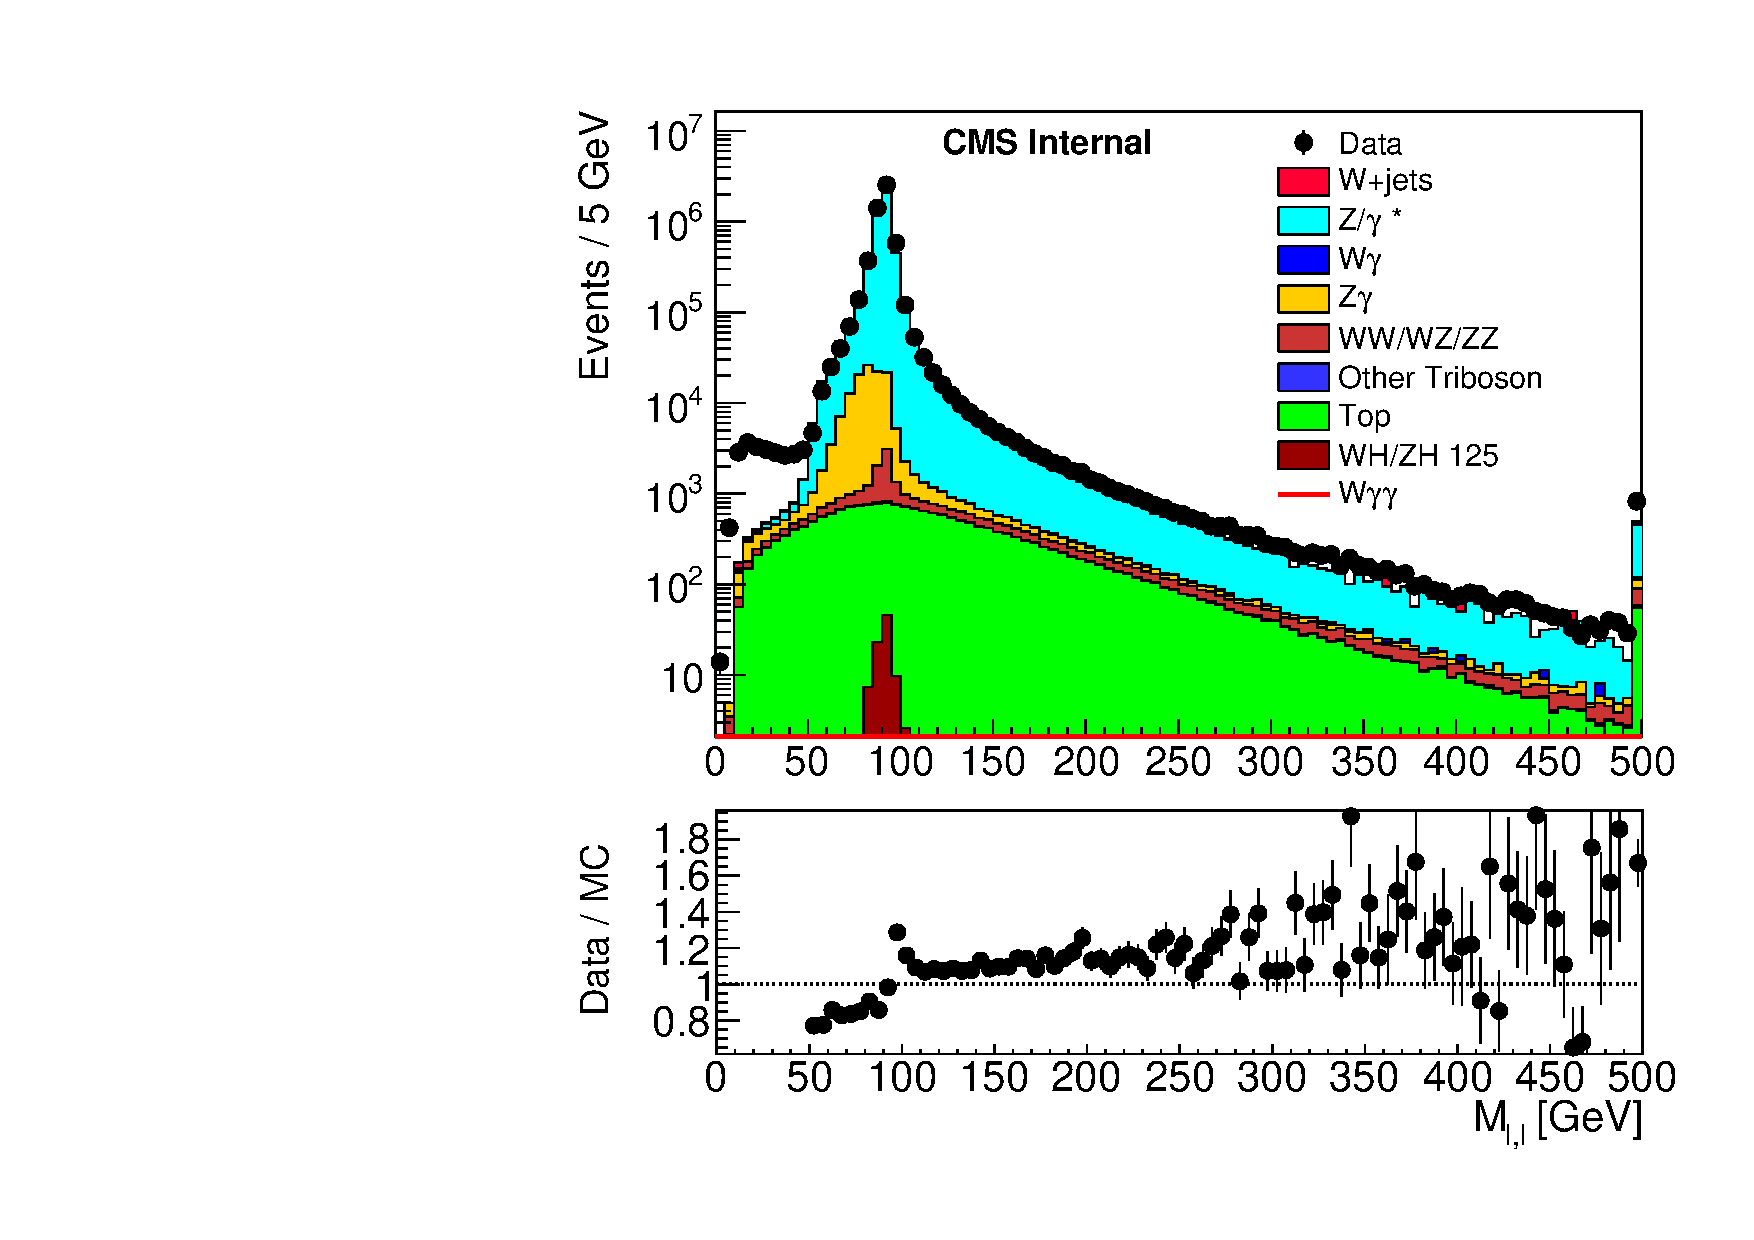
\includegraphics[width=0.8\textwidth]{Plots/m_leplep_2el.pdf}


         \column{0.5\textwidth}

         muon channel
        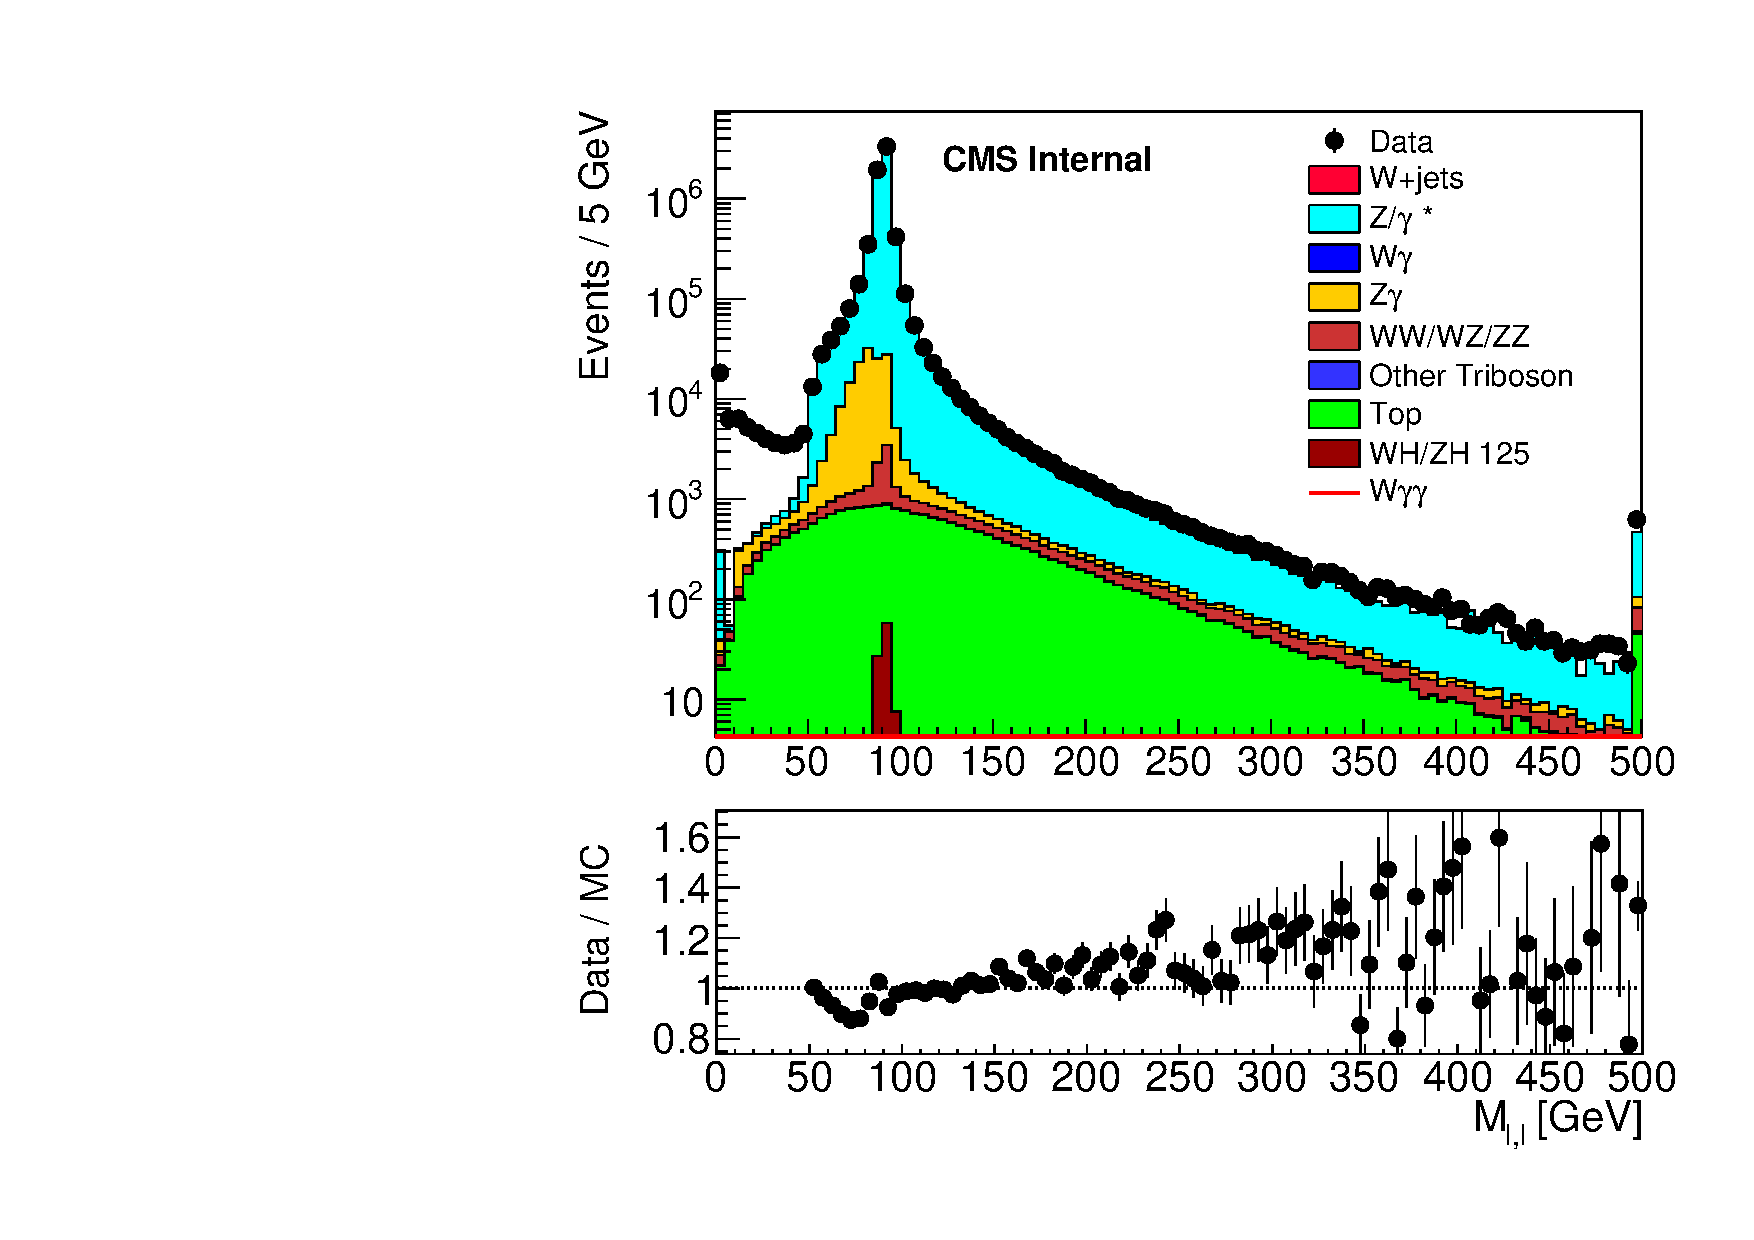
\includegraphics[width=0.8\textwidth]{Plots/m_leplep_2mu.pdf}

    \ec
}

\fr{ Z+$\gamma$ control region } {

    \begin{itemize}
        \item These plots show overlap between $Z\gamma$ and Z+jets samples
    \end{itemize}

    \bc
         \column{0.5\textwidth}
     
         electron channel
             
         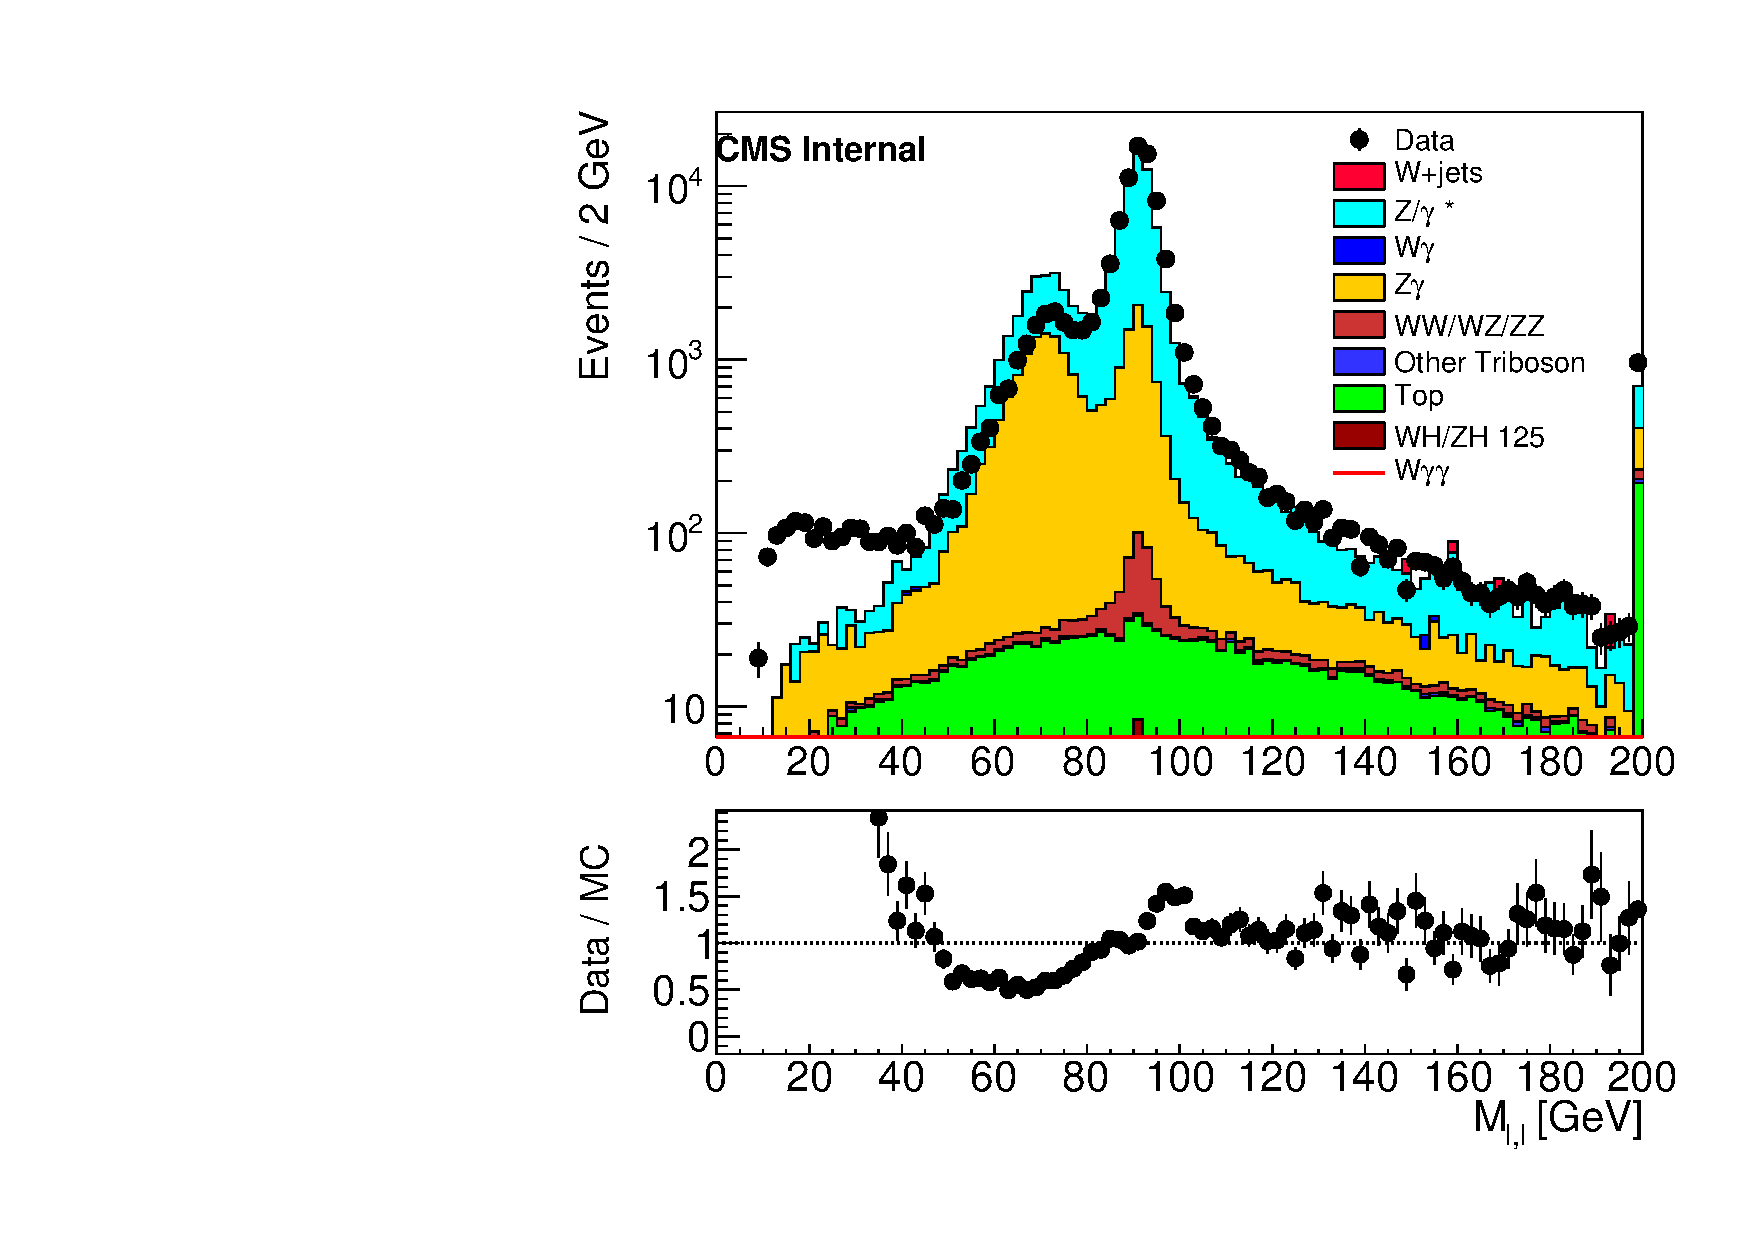
\includegraphics[width=0.8\textwidth]{Plots/m_leplep_2el1ph_noolaprm.pdf}


         \column{0.5\textwidth}

         muon channel
        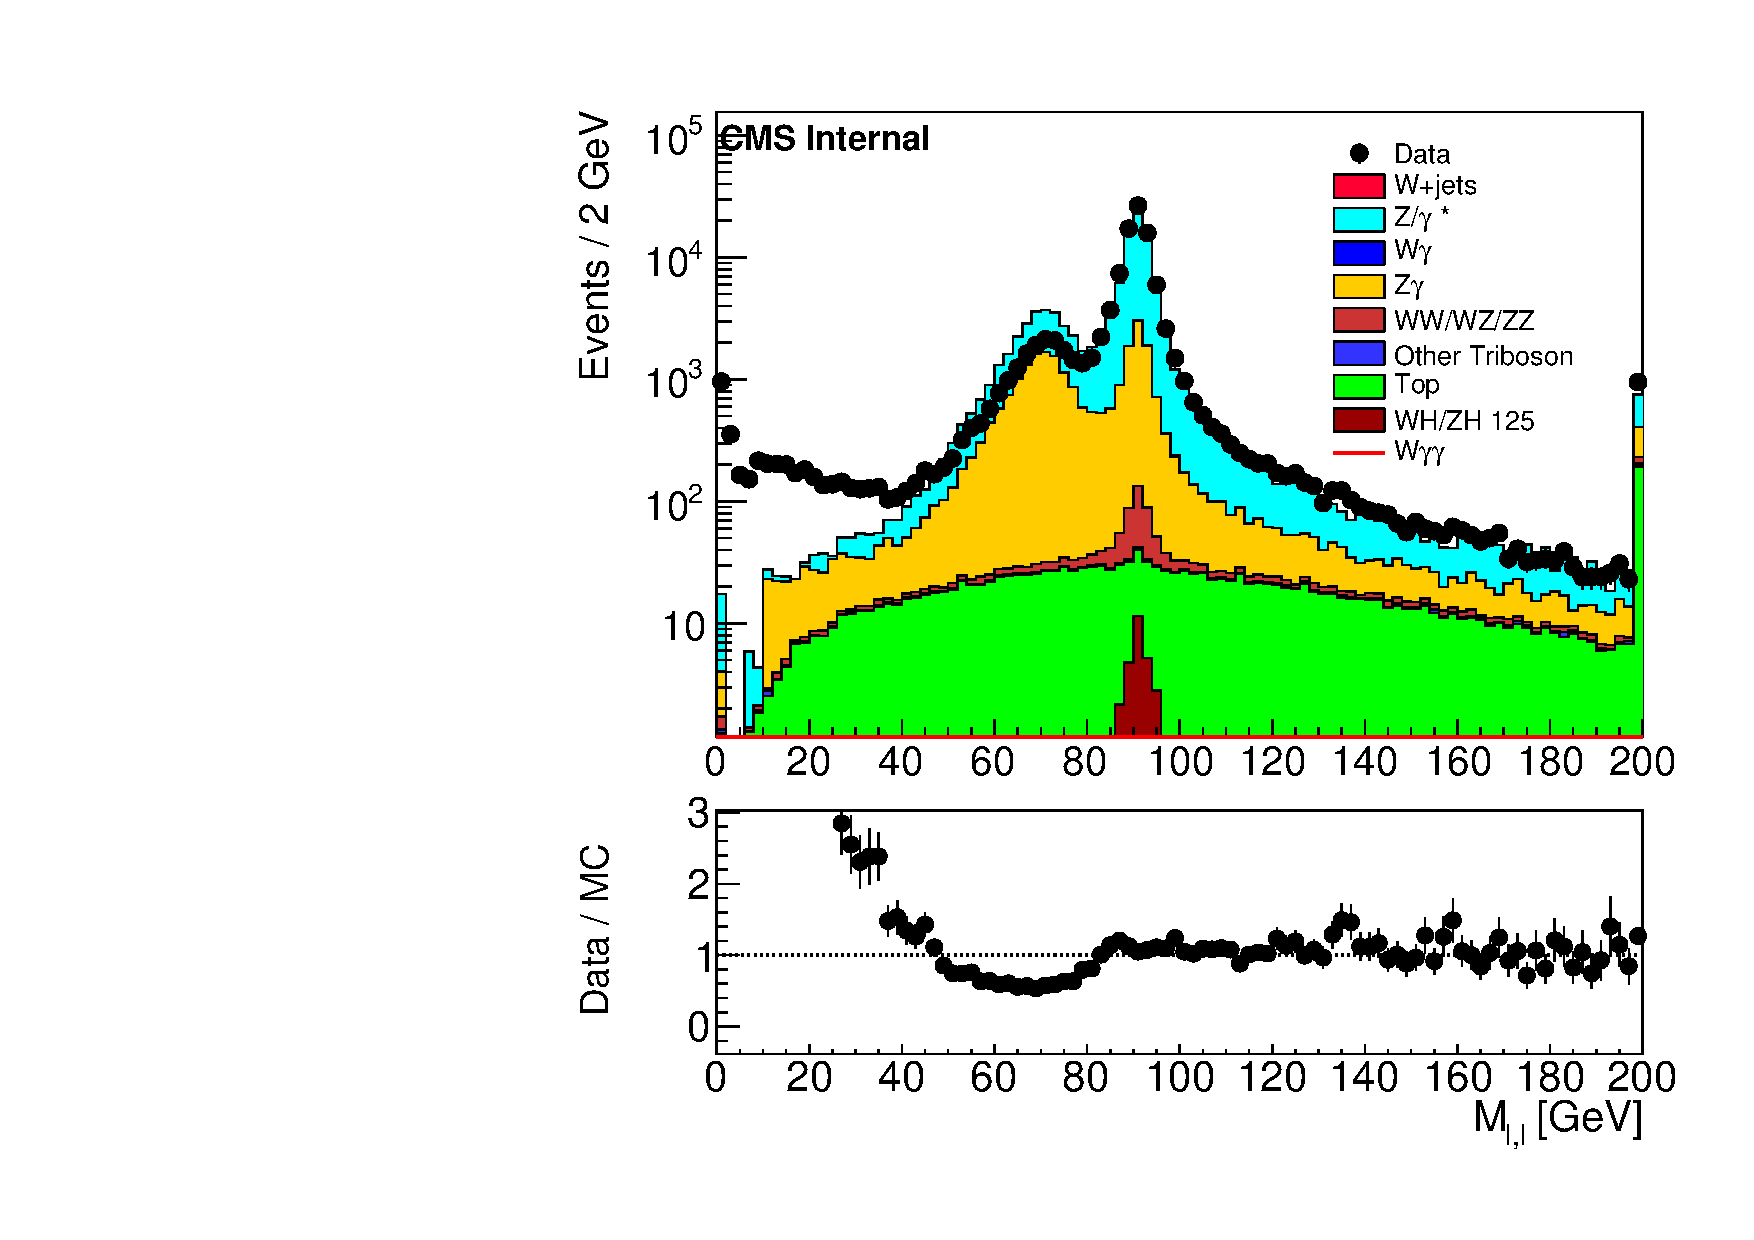
\includegraphics[width=0.8\textwidth]{Plots/m_leplep_2mu1ph_noolaprm.pdf}

    \ec
}

\fr{ Z+$\gamma$ control region } {

    \begin{itemize}
        \item Agreement is better after photon overlap removal
        \item The same overlap removal is applied to W+jets and W$\gamma$ samples
    \end{itemize}

    \bc
         \column{0.5\textwidth}
     
         electron channel
             
         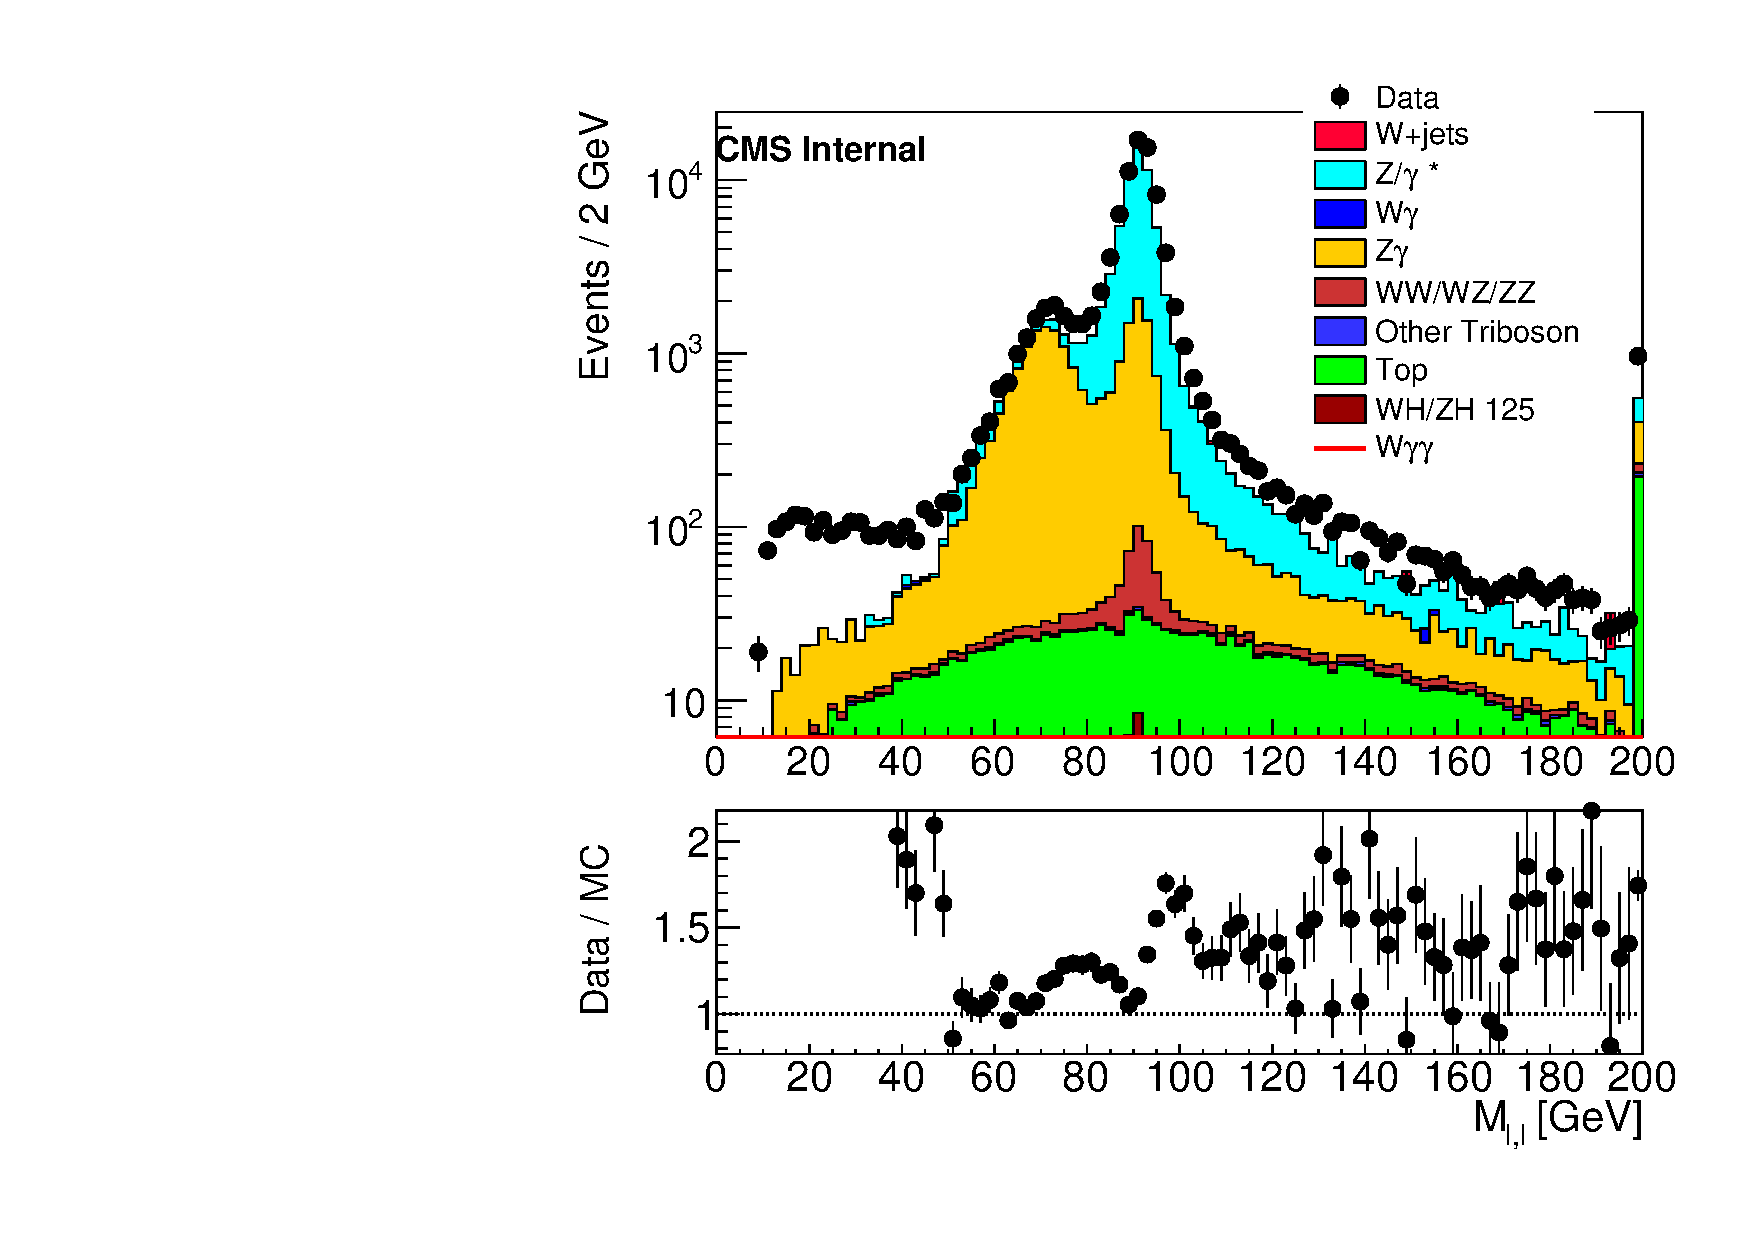
\includegraphics[width=0.8\textwidth]{Plots/m_leplep_2el1ph_witholaprm.pdf}


         \column{0.5\textwidth}

         muon channel
        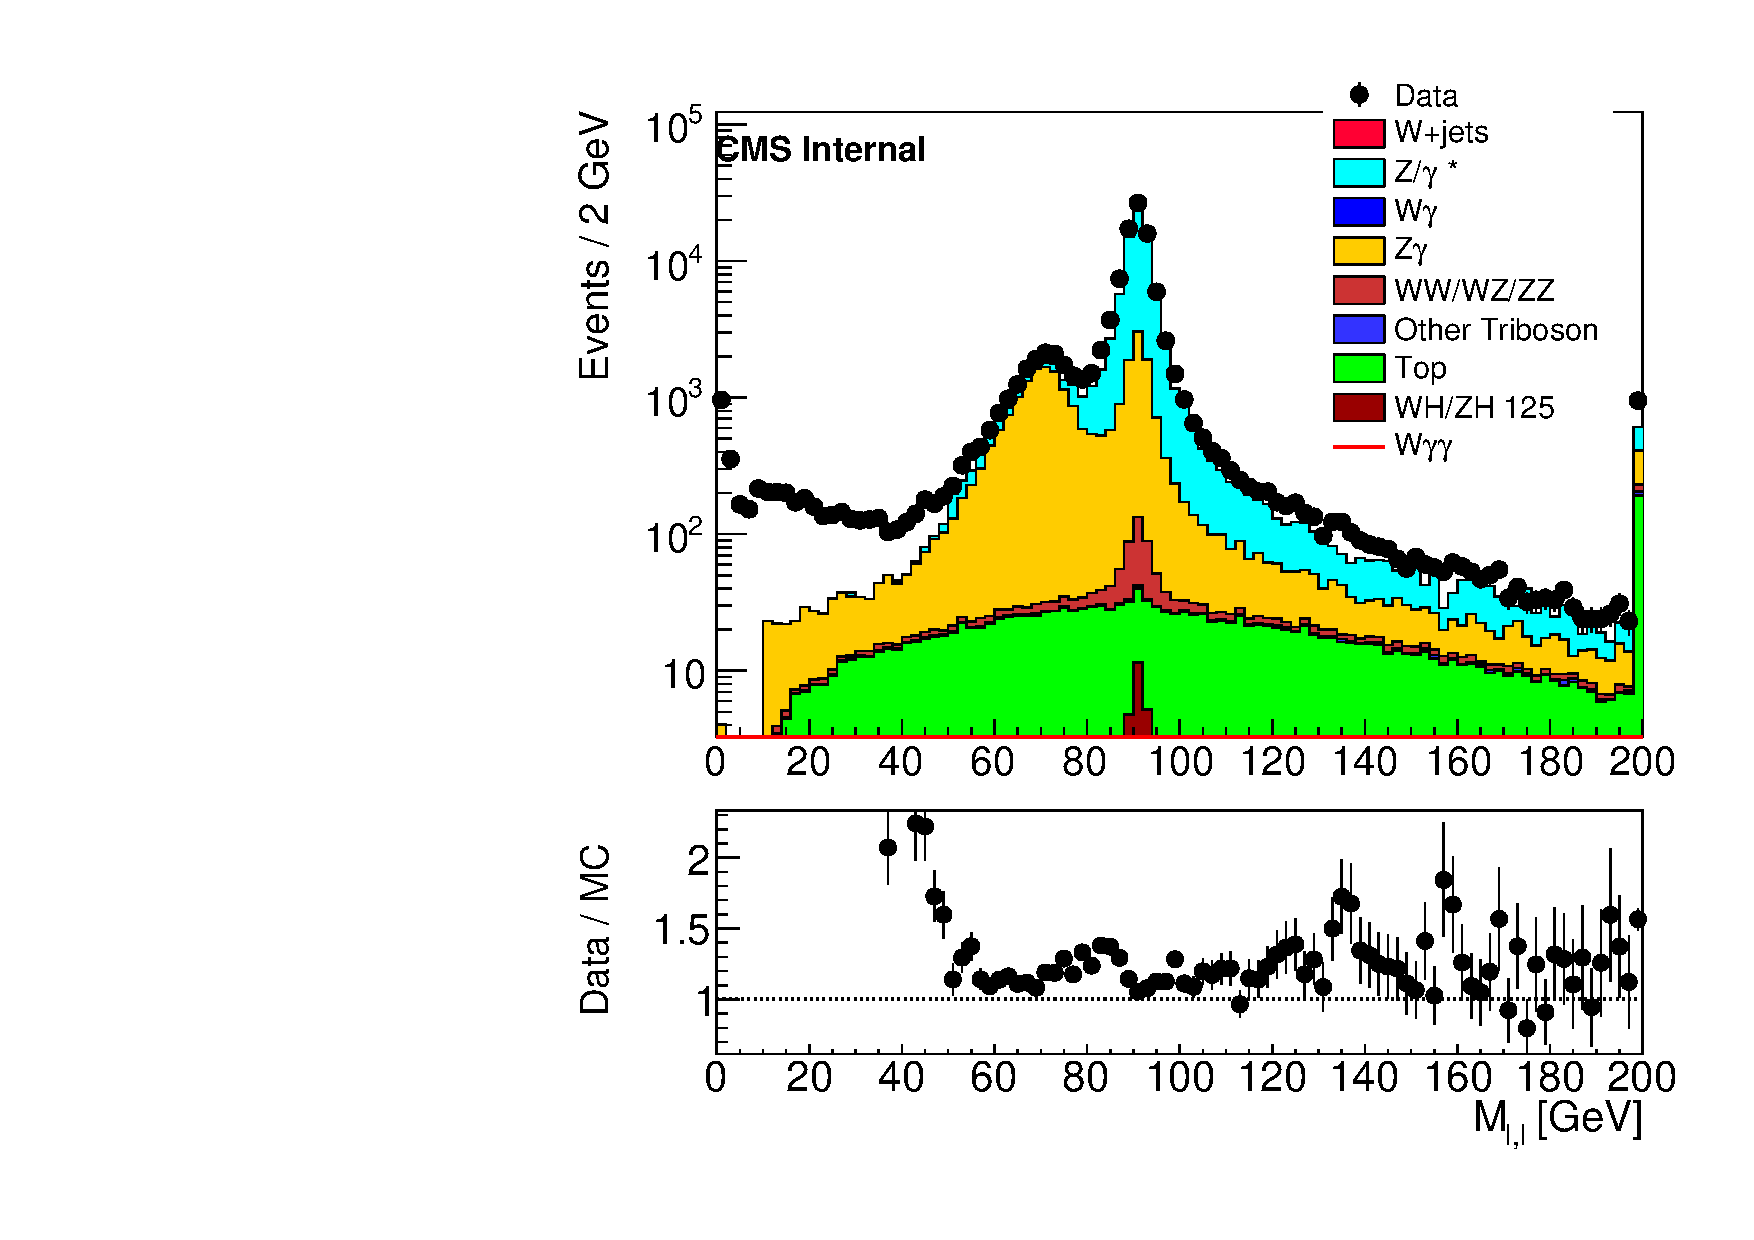
\includegraphics[width=0.8\textwidth]{Plots/m_leplep_2mu1ph_witholaprm.pdf}

    \ec
}

\fr{ Lepton + photon control regions } {


    \begin{itemize}
        \item Large contributions from Ws as expected
        \item Some disagreement between data and MC -- will investigate
    \end{itemize}

    \bc
         \column{0.5\textwidth}
     
         electron channel
             
         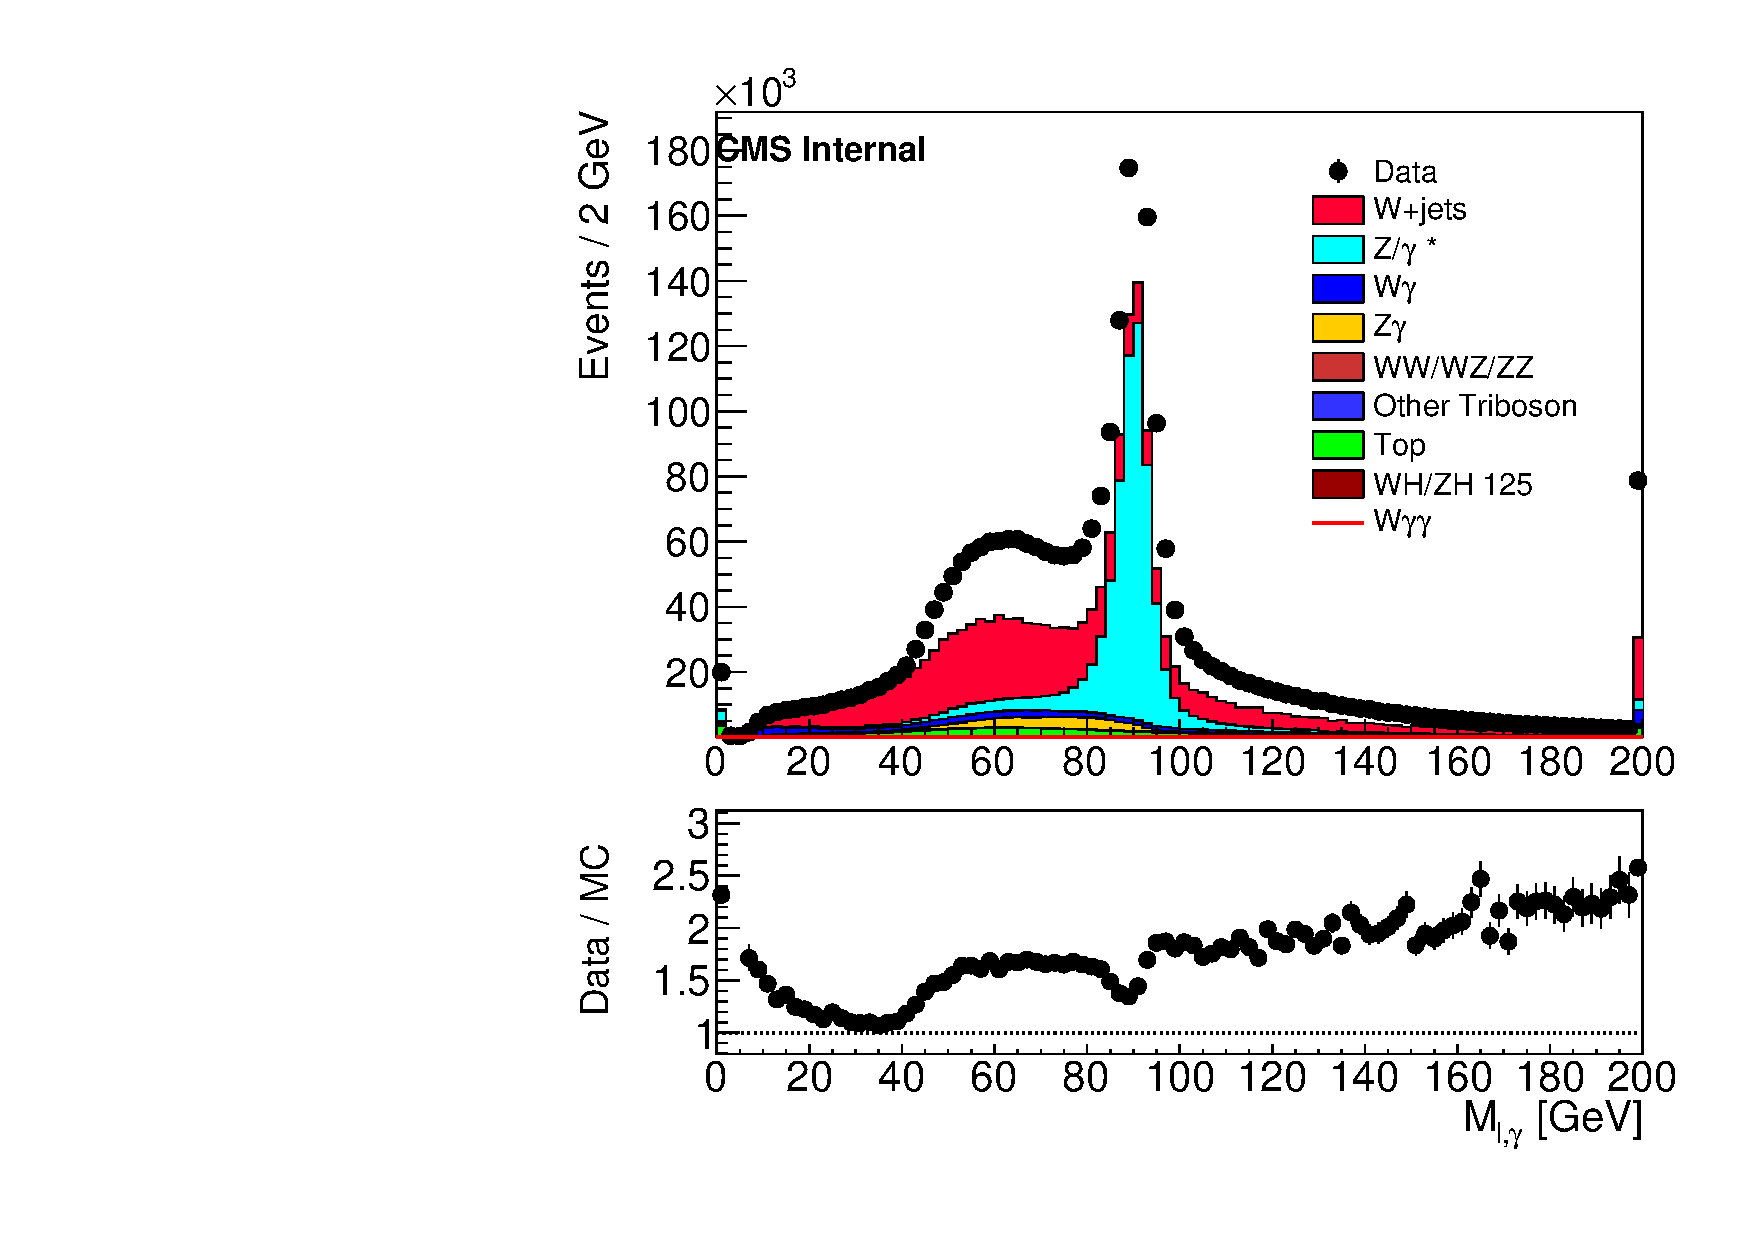
\includegraphics[width=0.8\textwidth]{Plots/m_lepph_1el1ph.pdf}


         \column{0.5\textwidth}

         muon channel
        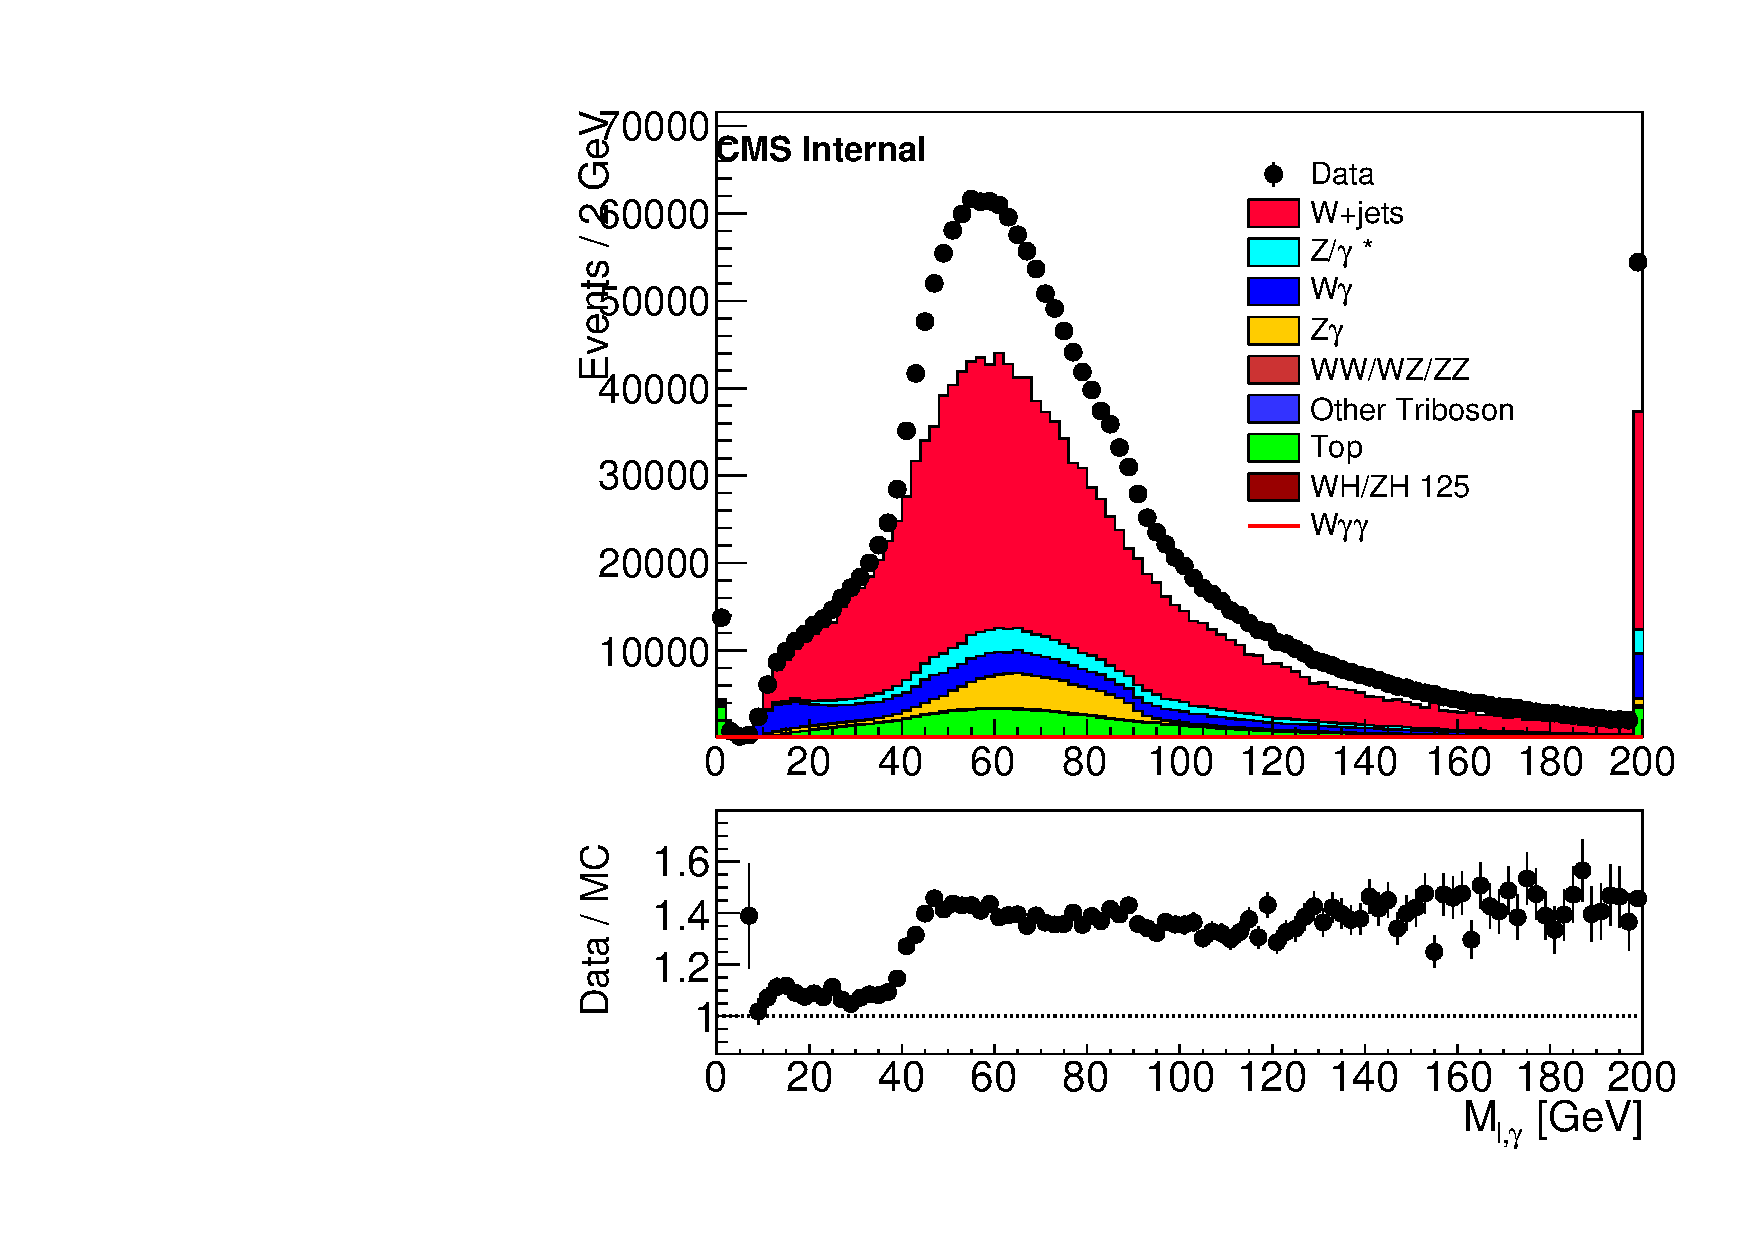
\includegraphics[width=0.8\textwidth]{Plots/m_lepph_1mu1ph.pdf}

    \ec

}

\fr{ Signal region -- photon $\Delta R$} {


    \begin{itemize}
        \item Two identified photons tend to be very close in many caases
        \item In the following plots, require $\Delta R > 0.2$
    \end{itemize}

    \bc
         \column{0.5\textwidth}
     
         electron channel
             
         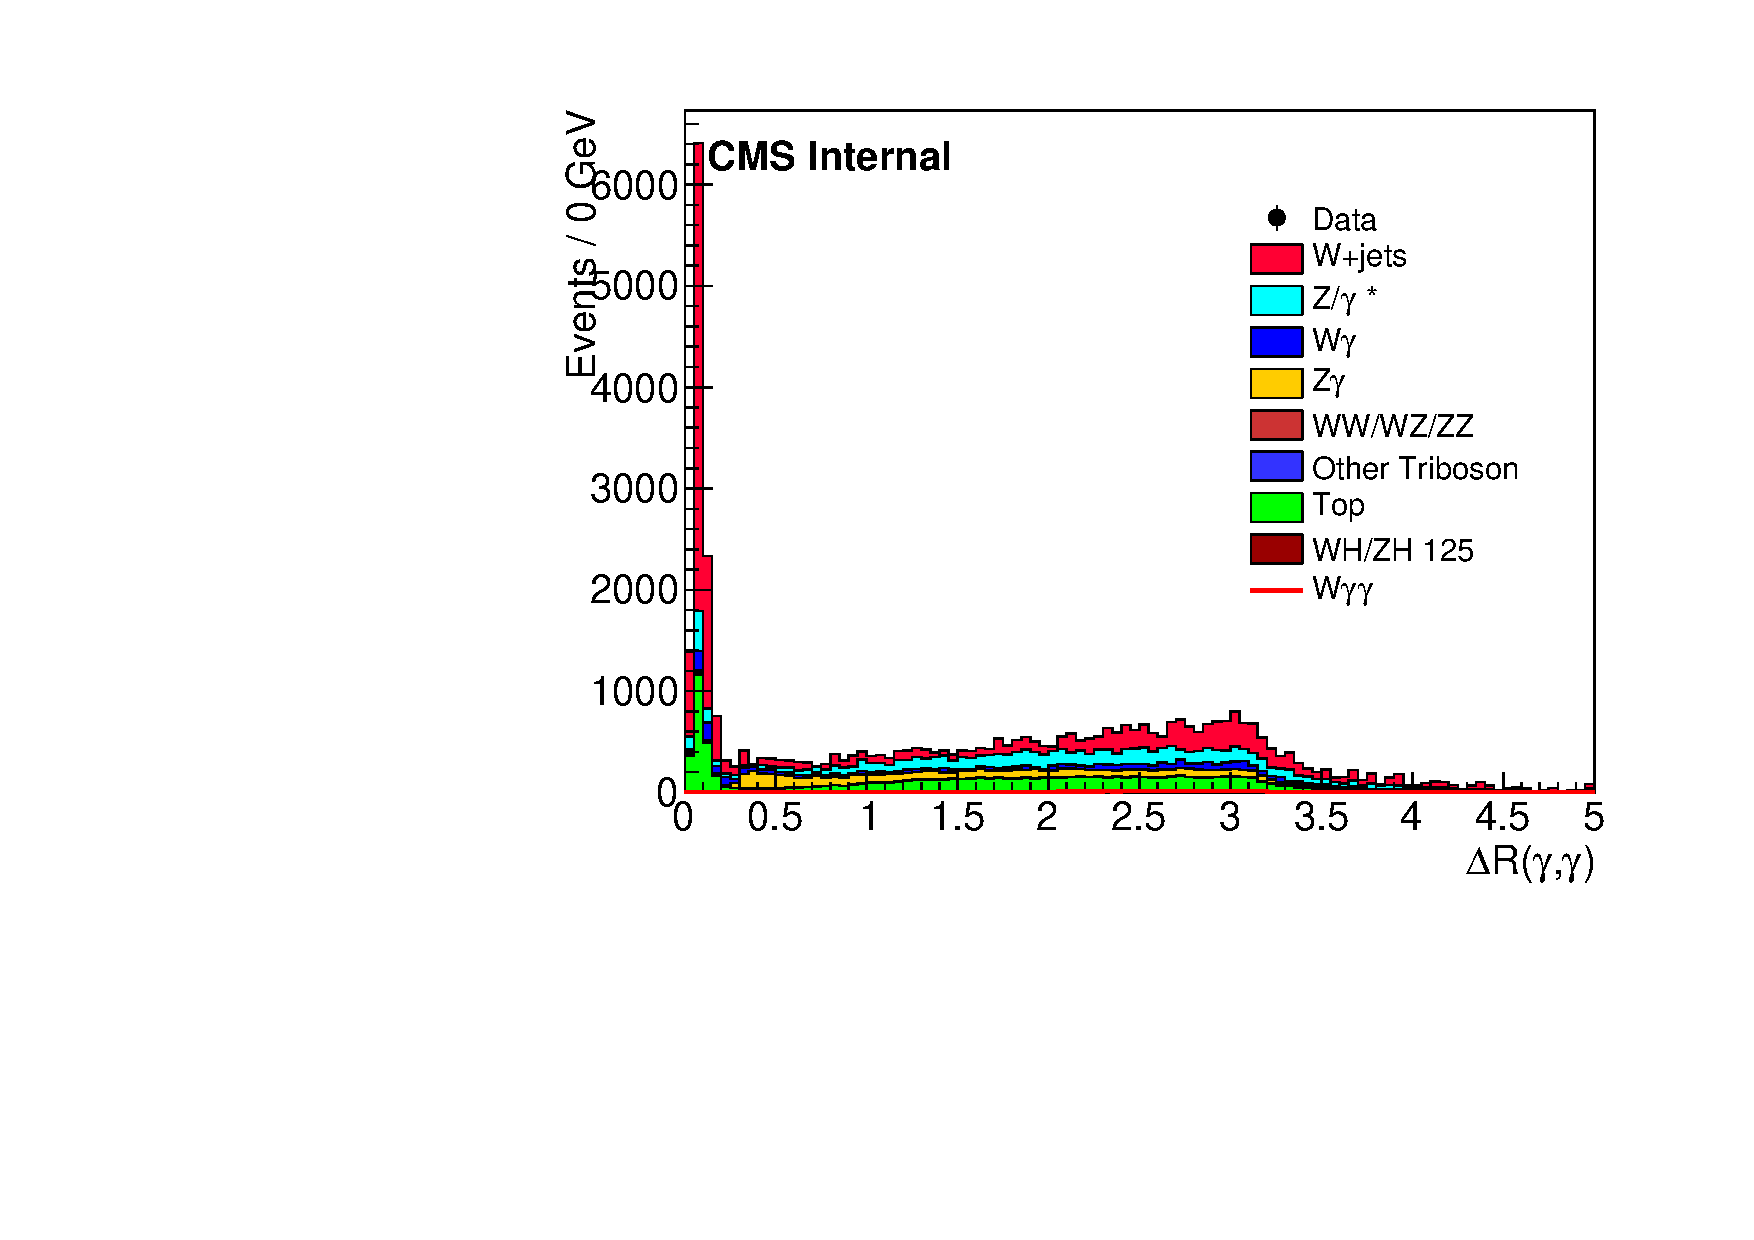
\includegraphics[width=0.8\textwidth]{Plots/DRPhPh_1el2ph.pdf}


         \column{0.5\textwidth}

    \ec

}

\fr{ Signal region } {


    \begin{itemize}
        \item Still large contributions from Ws
        \item The W background seems to be larger than before.  Difference is possibly caused by using loose photons
    \end{itemize}

    \bc
         \column{0.5\textwidth}
     
         electron channel
             
         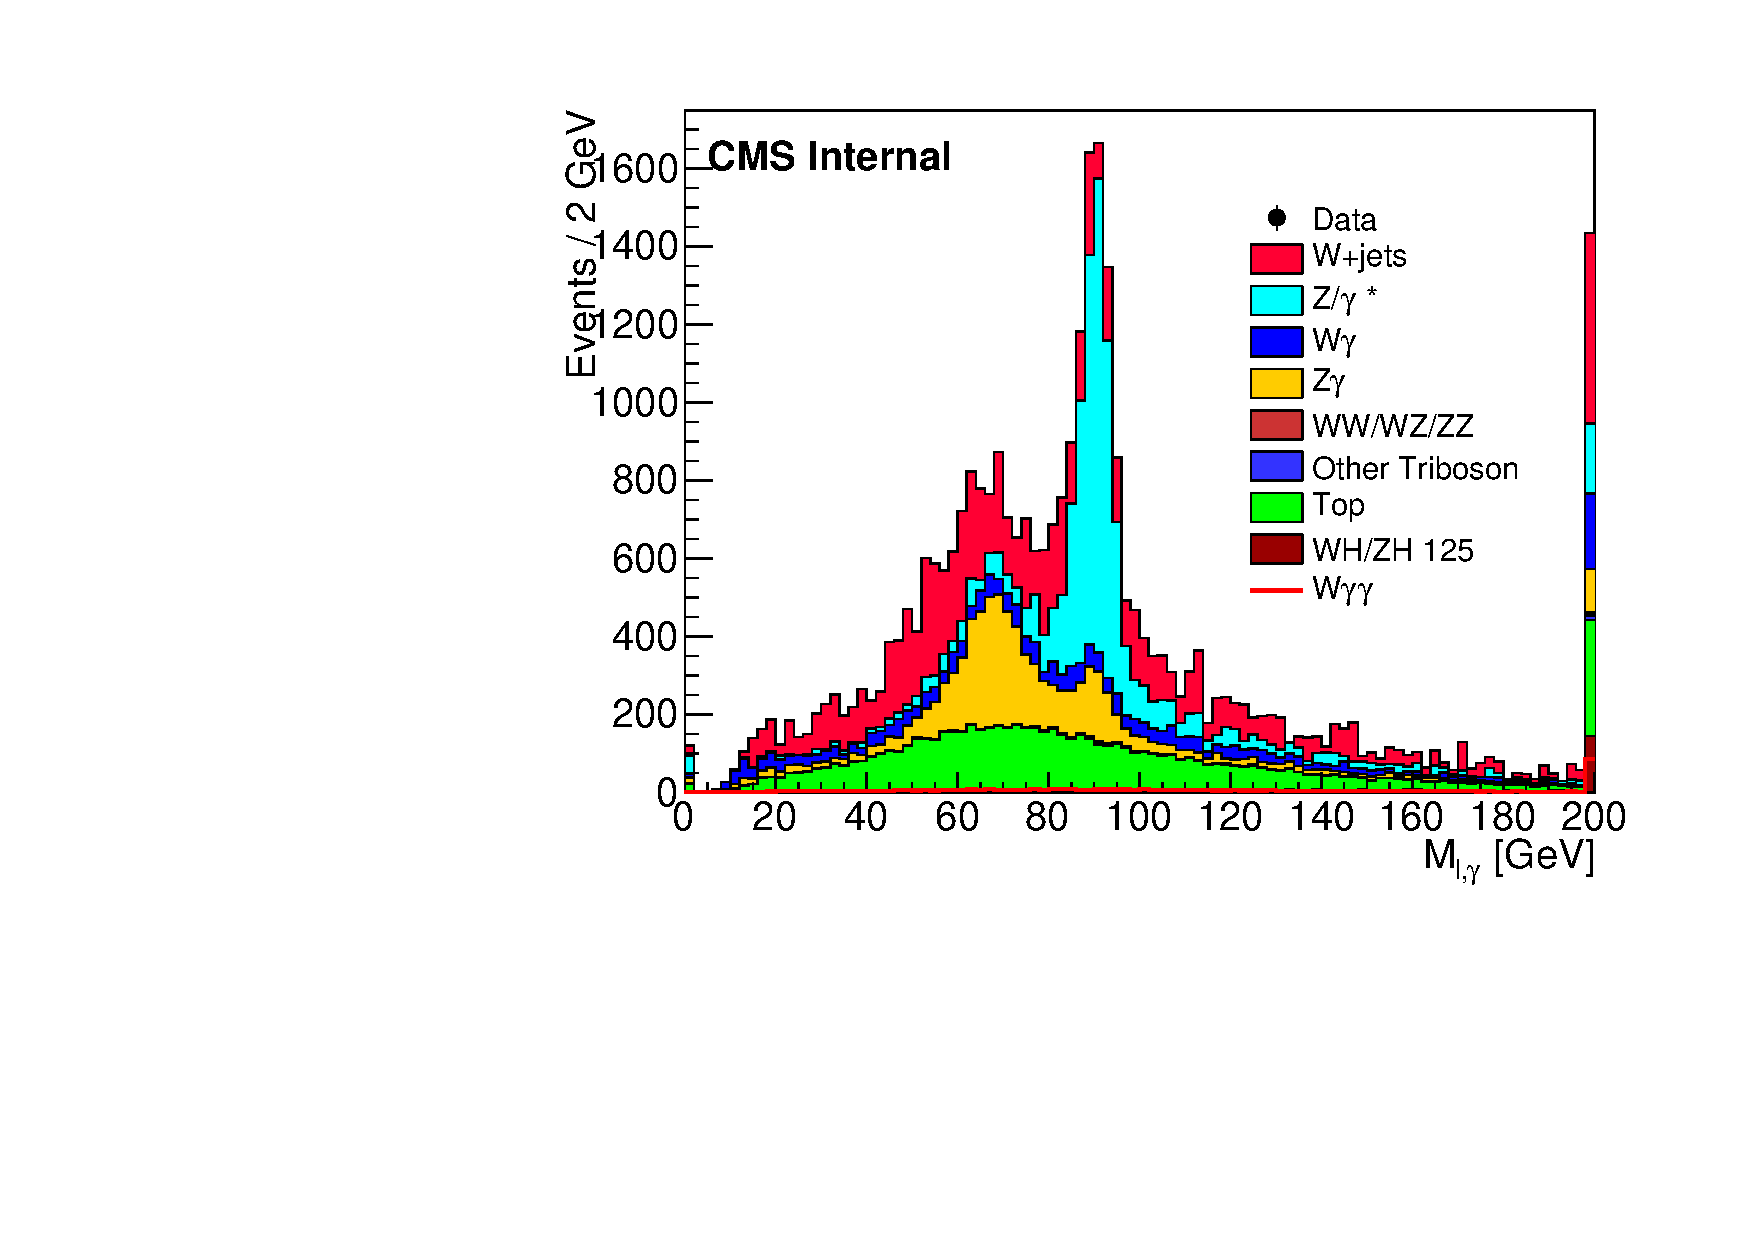
\includegraphics[width=0.8\textwidth]{Plots/m_lepph_1el2ph.pdf}


         \column{0.5\textwidth}

         muon channel
        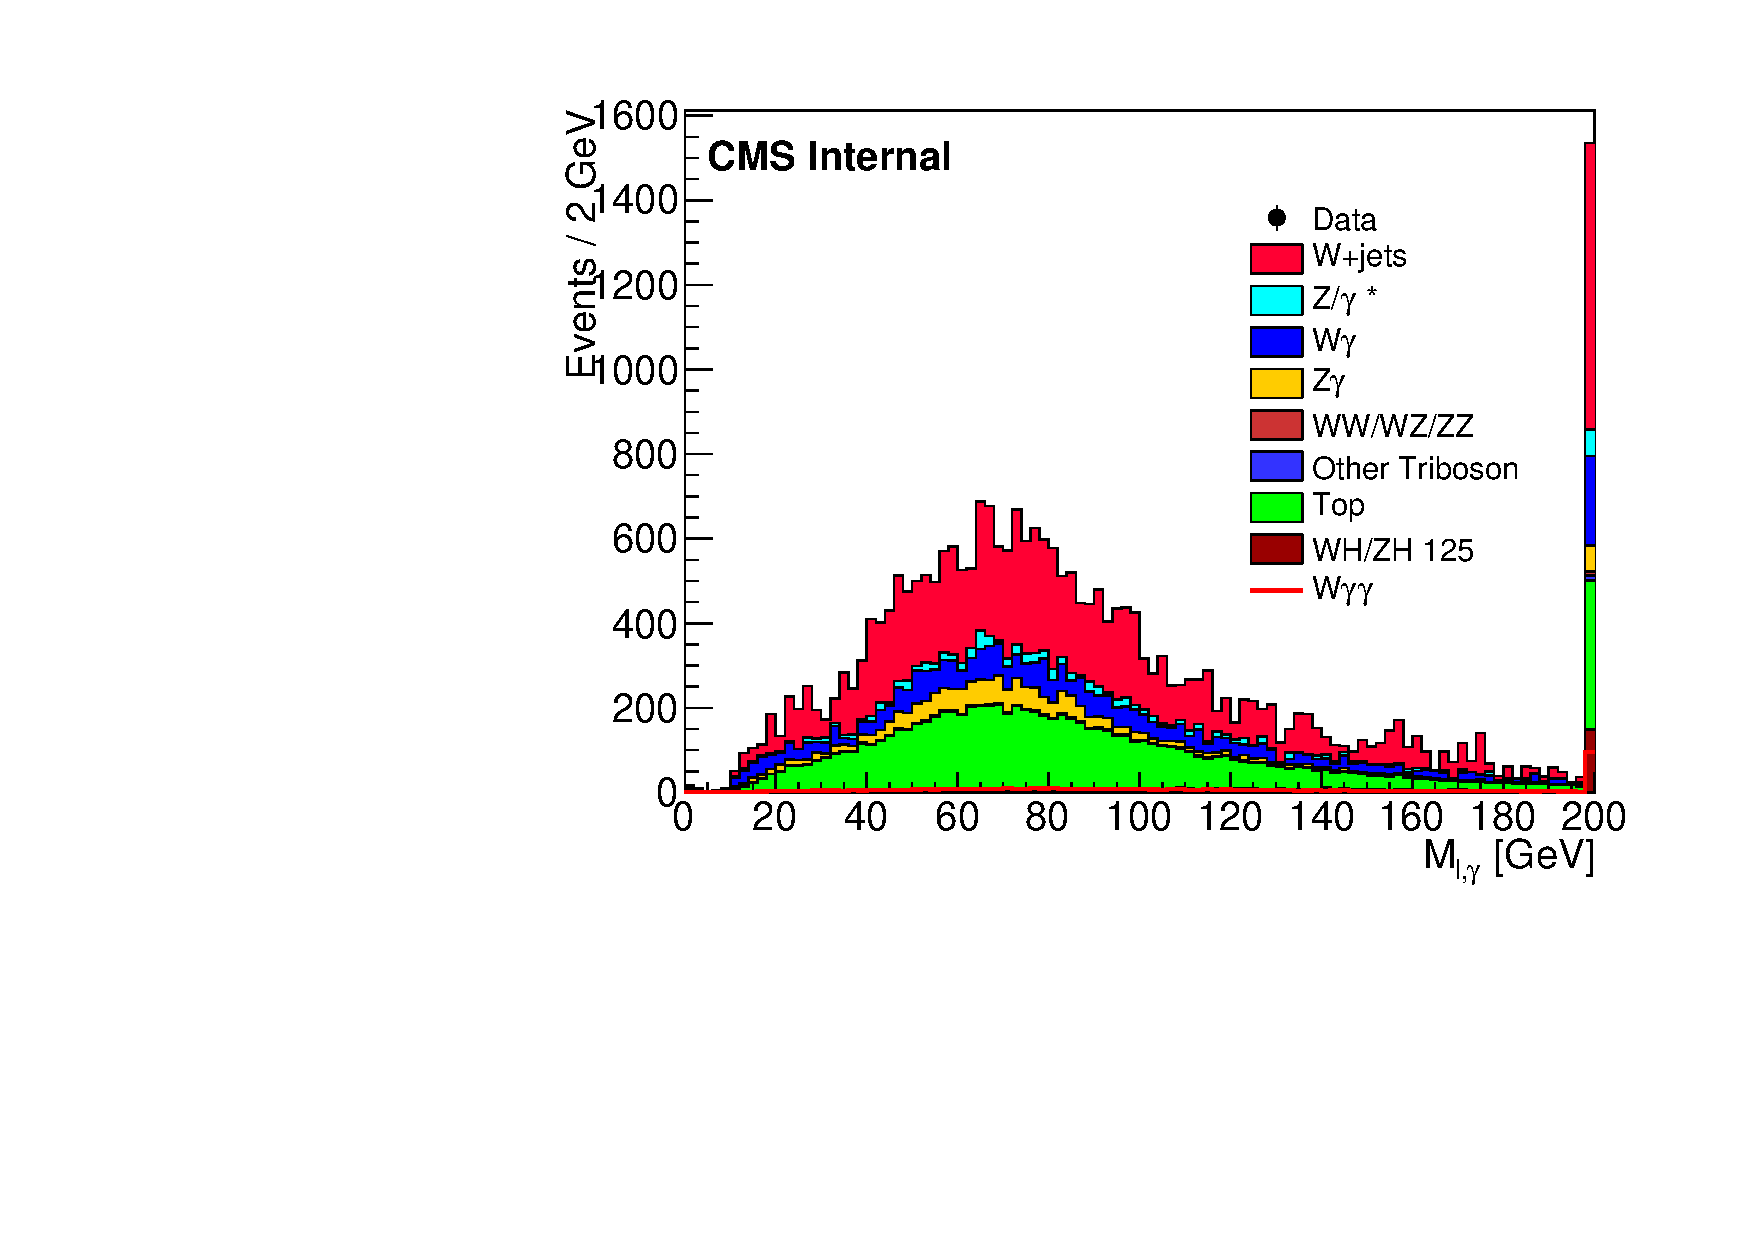
\includegraphics[width=0.8\textwidth]{Plots/m_lepph_1mu2ph.pdf}

    \ec

}


\fr{ Event Yields -- muon channel} {

    \scriptsize

    \begin{tabular}{l | l | l | l | l |}
    Sample    & Pass trigger & 1 $\mu$   & 1 $\mu$ + 1 $\gamma$ & 1 $\mu$ + 2 $\gamma$ \\
    Wjets     & 174043241    & 84468551     & 1048278   &  11630                       \\
    Zjets     & 27331241     & 13726436     & 90148     &  956                       \\
    W$\gamma$ & 1689770      & 796705       & 131275    &  3426                       \\
    Z$\gamma$ & 828157       & 410840       & 87177     &  1831                       \\
    Top       & 2044336      & 994788       & 127756    &  8360                       \\
    DiBoson   & 95580        & 52738        &  2985     &  77                       \\
    TriBoson  & 7417         & 3655         & 1101      &  83                       \\
    VH        & 3269         & 1079         & 284       &  634                       \\
    Total Bkg & 206055095    & 100460423    & 1491078   &  27591                 \\
    Data      & 140597517    & 62264753     &  2015926  &  --                    \\
    Signal    & 12081        & 5628         &  2070     &  590                   \\
    \end{tabular}

}

\fr{ Event Yields -- electron channel } {

    \scriptsize
    \begin{tabular}{l | l | l | l | l |}
    Sample    & Pass trigger & 1 $e$   & 1 $e$ + 1 $\gamma$ & 1 $e$ + 2 $\gamma$ \\
    Wjets     & 174043241    & 76771860  & 826026  & 9842                        \\
    Zjets     & 27331241     & 12670317  & 656650  & 7625                        \\
    W$\gamma$ & 1689770      &  742886   & 104568  & 2804                        \\
    Z$\gamma$ & 828157       & 385567    & 80116   & 5197                        \\
    Top       & 2044336      & 1122991   & 110510  & 7129                        \\
    DiBoson   & 95580        & 52693     & 2813    & 89                        \\
    TriBoson  & 7417         & 4061      & 994     & 68                        \\
    VH        & 3269         & 2273      & 432     & 523                        \\
    Total Bkg & 206055095    & 91758693  & 1783904 & 33788                        \\
    Data      & 140597517    & 70411234  & 2851959 &   --                      \\
    Signal    & 12081        & 6041      & 1791    & 506                        \\
    \end{tabular}
}

\fr{ summary } {

    \begin{itemize}
        \item First quick look at control regions and signal region with new ntuples
        \item A few bugs still have to be worked out with sample normalization and data/mc discrepancies
        \item Next steps : apply object momentum corrections, continue with studies of electrons faking photons
    \end{itemize}
}


\end{document}

